\section{ASCbase::Psuedo\-Lig\-Rmsd Class Reference}
\label{classASCbase_1_1PsuedoLigRmsd}\index{ASCbase::PsuedoLigRmsd@{ASCbase::PsuedoLigRmsd}}
{\tt \#include $<$Psuedo\-Lig\-Rmsd.H$>$}

Inheritance diagram for ASCbase::Psuedo\-Lig\-Rmsd::\begin{figure}[H]
\begin{center}
\leavevmode
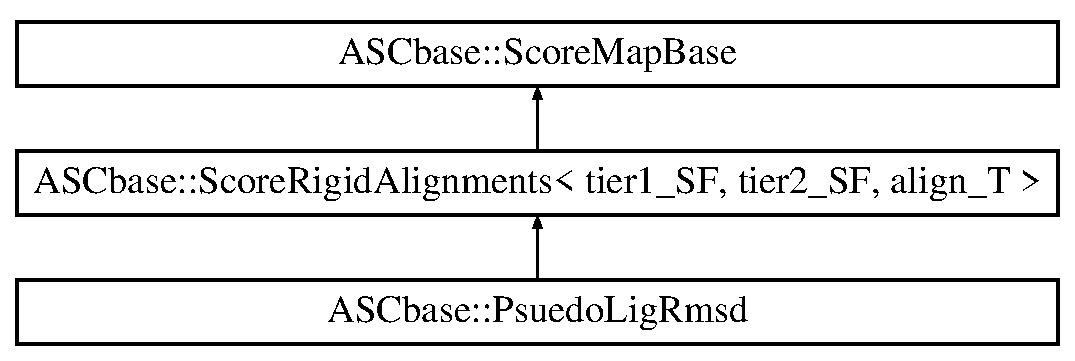
\includegraphics[height=3cm]{classASCbase_1_1PsuedoLigRmsd}
\end{center}
\end{figure}
\subsection*{Public Member Functions}
\begin{CompactItemize}
\item 
\bf{Psuedo\-Lig\-Rmsd} (\bf{Model\-Sitemap} $\ast$model\_\-in, const \bf{Search\-Parameters} \&params)\label{classASCbase_1_1PsuedoLigRmsd_cb2260f005103d3160c017839c4bd06e}

\begin{CompactList}\small\item\em Loads the model ligand and calls base cstr. \item\end{CompactList}\item 
\bf{$\sim$Psuedo\-Lig\-Rmsd} ()\label{classASCbase_1_1PsuedoLigRmsd_2ab21999e1e371a9eaa2839251d15d12}

\begin{CompactList}\small\item\em basic destruction \item\end{CompactList}\end{CompactItemize}
\subsection*{Protected Member Functions}
\begin{CompactItemize}
\item 
my\_\-float\_\-t \bf{score} (const \bf{Dbase\-Sitemap} \&search, rigid\_\-align\_\-vi scores)
\begin{CompactList}\small\item\em Given an alignment of search to the query, score said alignment. \item\end{CompactList}\item 
my\_\-float\_\-t \textbf{correspondences} (my\_\-float\_\-t $\ast$$\ast$query\_\-pts\_\-ptr, my\_\-float\_\-t $\ast$$\ast$db\_\-pts\_\-ptr, size\_\-t $\ast$npts)\label{classASCbase_1_1PsuedoLigRmsd_69e79ac94abe9233c291ecaccc6cae2e}

\end{CompactItemize}
\subsection*{Private Attributes}
\begin{CompactItemize}
\item 
\bf{mol2File} $\ast$ \textbf{model\_\-lig}\label{classASCbase_1_1PsuedoLigRmsd_c2c74580d19f2a232ad85eec12641ebe}

\end{CompactItemize}
\subsection*{Static Private Attributes}
\begin{CompactItemize}
\item 
static const std::string \bf{\_\-fname} = \char`\"{}Psuedo\-Lig\-Rmsd.C\char`\"{}\label{classASCbase_1_1PsuedoLigRmsd_2f21de3bff3a23947a0f443dd906c0bc}

\begin{CompactList}\small\item\em \char`\"{}Psuedo\-Lig\-Rmsd.C\char`\"{} \item\end{CompactList}\end{CompactItemize}


\subsection{Detailed Description}
NOTE: this method only works for ligands which are EXACTLY the same. That is the corresponding atom for the nth query ligand atom is the nth target ligand atom. 



\subsection{Member Function Documentation}
\index{ASCbase::PsuedoLigRmsd@{ASCbase::Psuedo\-Lig\-Rmsd}!score@{score}}
\index{score@{score}!ASCbase::PsuedoLigRmsd@{ASCbase::Psuedo\-Lig\-Rmsd}}
\subsubsection{\setlength{\rightskip}{0pt plus 5cm}my\_\-float\_\-t Psuedo\-Lig\-Rmsd::score (const \bf{Dbase\-Sitemap} \& {\em search}, rigid\_\-align\_\-vi {\em scores})\hspace{0.3cm}{\tt  [protected]}}\label{classASCbase_1_1PsuedoLigRmsd_889f9461ef48612a4d146c4b7c34b46c}


Given an alignment of search to the query, score said alignment. 

\begin{Desc}
\item[Parameters:]
\begin{description}
\item[{\em search}]Pointer to the sitemap aligned to the model sitemap \end{description}
\end{Desc}
\begin{Desc}
\item[Returns:]The score of the alignment \end{Desc}


The documentation for this class was generated from the following files:\begin{CompactItemize}
\item 
Psuedo\-Lig\-Rmsd.H\item 
Psuedo\-Lig\-Rmsd.C\end{CompactItemize}
